%To get a sideways table with wrapped text there are 2 options
%1. \begin{sideways} Content to rotate. \end{sideways}
%2. \afterpage{ \begin{landscape} Content to rotate. \end{landscape}
%Use afterimage for now.


\chapter{Selection of \bsmumu events for the effective lifetime Measurement}
\label{selection_chapter}
The analysis described in Chapter X for the \bsmumu effective lifetime requires \bsmumu and \bhh decays to be identified in the data sets recorded by the LHCb experiment. Although \bsmumu decays leave a clear 2 muon signature in the detector, the selection of these decays is challenging because it is a very rare process and there are many other processes that can mimic a \BsMuMu decay in the detector. The background processes are described in Section~\ref{sec:backgroundoutline}. To understand different aspects of the selection and analysis of \BsMuMu decays, particle decays with a similar topology to \BsMuMu are used. \bhh decays, where $h = K, \pi$, are used because they have large branching fractions and are well understood from previous LHCb analyses as well as a similar topology to \bsmumu decays. 
%The selection of \bhh decays is kept as close as possible to the selection of \bsmumu so they can be used as a validation channels.
The measurement of the \bmumu Branching Fractions, described in Chapter X, requires the use of \bujpsik decays, as well as \bmumu and \bhh decays, to be used as a normalisation channel.
This Chapter describes the selection of \bmumu, \bhh and \bujpsik decays for the effective lifetime and Branching fraction analyses. The analyses share many of the same selection requirements. The selection occurs in several stages, and the development of the selection relies on simulated events which are detailed in Section~\ref{sec:MCsamples}. The first step to select decays is choosing what requirements to place on the trigger which is followed by a set of loose selection requirements to remove obvious background events. These two steps are described in Sections~\ref{sec:triggerRequirements} and \ref{sec:stripping}. A tighter selection is applied to the output of the stripping as described in Section~\ref{sec:offline_sel} and particle identification requirements are used in Section~\ref{sec:PID} to further reduced background events. Finally a multivariate classifier is described in Section~\ref{sec:BDT} used as the final step in the selection to reduced the backgrounds to a level suitable for the analysis in Chapter X to be preformed. Throughout this Chapter \bsmumu and \bdmumu are selected in the same way.

The LHCb collaboration has published a number of papers studying the \bsmumu decay, the selection described in this Chapter has been built up over a number of years by a range of different collaboration members. The studies detailed in sections X, X and Y was done for this thesis.





\section{Backgrounds}
\label{sec:backgroundoutline}
%A \bs decaying into two muons leaves information in the LHCb detector with certain identifying characteristics. The two muons form a good vertex that is displaced from the primary vertex of the event because the Bs has a long lifetime and the combined momentum of the muons can be extrapolated backwards to the primary vertex because the muons are the only decay products of the \bs. There are other processes that occur in proton-proton decays that can leave information in the detector in a similar pattern to \bsmumu decays. The reconstruction, described in Section X, produces many \bsmumu candidates, the aim of the selection is to separate the real \bsmumu decays from the background in the reconstructed candidates.

%The background sources for \bsmumu decays can be split into two groups, those that have quite obvious difference from \bsmumu decays and those that do not. The first set can be removed from the data set by taking advantage of the obvious differences whilst keeping a high 

The reconstruction process, outlined in Section X, produces numerous \bsmumu candidates from pairs of muons created by $pp$ collisions and recorded in the detector. Some candidates will have come from real \bsmumu decays but there are other processes that occur during $pp$ collisions that can create two muons that when combined look a lot like a \bsmumu decay. %In the detector a \bsmumu decay will produce two muons that form a good vertex which is displaced from the primary vertex where the \bs was produced.   

%The selection aims to seperate real \bsmumu decyas from these background to produce a set of \bsmumu candidates with a high signal purity from which the \bs effective lifetime can be measured. (here?)
%The main sources of background processes for \bsmumu decays are;
The main sources of background decays that mimic \bsmumu decays are:
\begin{itemize}
\item Elastic collisions of protons that produce a pair of muons via the exchange of a photon, $pp \to p \mu^{+} \mu^{-} p$. The proton are travel down the beam pipe and are undetected leaving the muons to be reconstructed as \bsmumu. Typically the muons produced in this way have low transverse momentum. %whilst the protons travel down the beam pipe. The muons produced have low transverse momentum.
\item Inelastic proton collisions that create two muons at the primary vertex. The muons for a good vertex and are combined to for a \bs that decays instantaneously. This type of background is prompt combinatorial background. 
\item $B_{}^{0}\to\mu^{+}\mu^{-}\gamma$ decays where the photon is not reconstructed. The presence of the photon in the decay means that $B_{S}^{0}\to\mu^{+}\mu^{-}\gamma$ decays are not helicity suppressed and could therefore be a sizable background, however the photon gains a large transverse momentum resulting in the reconstructed \bs mass being much lower than expected.
\item Random combinations of muons produced by separate semi-leptonic decays. The \bsmumu candidates formed in this way are long lived combinatorial background because the reconstructed \bs will not decay instantaneously. %can be formed when muons produced in separated semi-leptonic decays are combined. These are known as long lived combinatorial background because the reconstructed \bs will not decay instantaneously.
\item Semi-leptonic decays where one of the decay products is mis-identified as a muon and/or is not detected. The resulting mass of the \bs candidate is lower than expected due to the missing particle information. The semi-leptonic decays that contribute to \bsmumu backgrounds in this way are \bdpimunu, \bsKmunu, \bpimumu, \bdpimumu and \bcjpsimunu where \jpsimumu.
\item \bhh decays, where $ h  = K, \pi$, where both hadrons are mis-identified as muons. This usually occurs when the hadrons decay in flight. Similarly to mis-identified semi-leptonic decays the reconstructed \bs candidate mass is lower than expected.
\item \bdmumu decays that are identical to \bsmumu decays apart from the difference in the $B$ meson masses. The \bd decay is irrelevant for the measurement of the \bsmumu effective lifetime and is therefore a background for this measurement.
\end{itemize}

The selection aims to separate real \bsmumu decays from the background to produce a set of \bsmumu candidates with a high signal purity from which the \bs effective lifetime can be measured. This is challenging because \bsmumu decays are highly suppressed decays therefore reconstructed candidates are predominately made from background decays.

%The \bdmumu is also a background process for measuring the \bsmumu effective lifetime, the only way to seperate \bsmumu and \bdmumu decays is by using the different masses of the \bs and $B^{0}$ mesons. (In the bullet points?)

%Maybe say how since the decay is so rare there are many many more reconstruced background decays than real bsmumu decays?

{\it I could put a plot showing the mass plot from the previous analysis or I could make a plot something like Siim has to illustrate what i mean but that feels a bit like copying!}
%Separating the backgrounds from the \bsmumu decays can be done relatively straightly forwardly for many of the background processes by taking advantage of the obvious differences between the background and \bsmumu decays. However, distinguishing \bsmumu decays from long lived combinatorial backgrounds, and mis-idetificed \bhh and semi-leptonic decays is more challenging and \bsmumu decays must be sacrificed in order to remove a sufficient about of the background processes for the analysis to be performed. For the effective lifetime analysis the \bdmumu decay is not relevant and is therefore a background, however since the decays are extremely similar the \bsd masses are the only way to seperate the decays.

\section{Simulated Particle Decays}
\label{sec:MCsamples}
Simulated particle decays, as described in Section X, are used to develop the selection and analysis of \bsmumu decays. Large clean samples of simulated decays are needed to separate signal decays from background decays and to understand the impact of selection criteria on decays present in data. 
%Many different simulated decay types have been used over time for the development of the selection and analysis of \bsmumu decays, 
The simulated decays used for studies documented in this thesis are listed in Table~\ref{tab:MC_decays} along with the data taking conditions and simulation versions used to generated the decays.

There exist multiple versions of the simulation because it is updated as understanding of the detector increases and to incorporate differences in data taking conditions, such as the trigger lines or center-of-mass energy, present in each year of data is collected. Similar simulation versions must be used to compare different types of simulated decays or data taking conditions so that differences are not masked by variations in the simulation of the decays. The simulated decays in Table~\ref{tab:MC_decays} listed under the studies they are used in. 

Simulated \bbbarmumux decays are used to understand the combinatorial background of \bsmumu decays, however producing a large enough sample of these decays to be useful is computational expensive and produces large output files to save generated decays. Therefore cuts are applied at the generation level for \bbbarmumux decays to reduce the size of the samples that are saved and to speed production. The cuts, listed in Table~\ref{tab:MC_decays}, are applied on the muon momenta, the reconstructed mass of the muon pair, the product of the momenta of the muons and the distance of closest approach of the two muon. %The generator level cuts save a factor of 5 of what needs to be saved, striping filtering also reduces it by a factor of 10! The information is in the LHCb-ANA-2013-032, the 2012 bbbarmumux sample corresponds to 7fb-1.
  
%The development of the selection and analysis of \bsmumu decays requires the use of simuluated decays, as described in Section X. The reconstucted \bsmumu candidates come for a range of different different processes, as already discussed, in order to seperate real \bsmumu decays from the background, large clean samples of simulated decays are used so that the differences between signal and background decays can be understood. Futhermore simulated samples are needed to understand 

 
\begin{table}[htb]
\begin{center}
%%\begin{tabular}{p{6cm}p{2.5cm}p{2cm}p{3cm}}                                                                                                           
\begin{tabular}{p{0.45 \textwidth}p{0.15 \textwidth}p{0.15 \textwidth}p{0.15 \textwidth}}
\hline
Decay 			& Data taking conditions 	& Simulation version 	& Generated events \\ \hline 
\multicolumn{4}{c}{{\it Stripping selection studies selection}}  \\ \hline 
\bsmumu			& 2012	& sim06b  		& 2 M			 \\ 
\bdmumu			& 2012	& sim06b  		& 2 M\\ 
\bdkpi			& 2012	& sim06b  		& 1 M\\ 
\bujpsik		& 2012	& sim06b  		& 1 M\\ \hline 
\multicolumn{4}{c}{{\it Multivariate classifier training}}  \\ \hline
\bbbarmumux, {\footnotesize p~$>$~3~\gevc, 4.7~$< M_{\mu^{+} \mu^{-} <$~6.0~\gevcc, DOCA~$<$~0.4mm, 1~$<$~PtProd~$<$~16~\gevc}
                        & 2012  & sim06b                & 8.0 M      \\
\bbbarmumux, {\footnotesize p~$>$~3~\gevc, 4.7~$< M_{\mu^{+} \mu^{-} <$~6.0~\gevcc, DOCA~$<$~0.4mm,   PtProd~$>$~16~\gevc}
                        & 2012  & sim06b                & 6.6 M\\
\bsmumu                 & 2012  & sim06b                & 2 M \\ \hline
\multicolumn{4}{c}{{\it Analysis method development}}  \\ \hline 
\bsmumu			& 2011 	& sim08a   		& 0.6 M		  \\ 
       			& 2012 	& sim08i  		& 2 M			 \\ 
        		& 2015	& sim09a  		& 2 M	 \\ 
        		& 2016	& sim09a  		& 2 M ? \\ %Is this correct? I thought in the ntuples we have a lot more 2015 than 2016 MC? 
\bdkpi			& 2011	& sim08b  		& 0.8 M  \\ %11102003
        		& 2012	& sim08g  		& 8.6 M \\ 
        		& 2015	& sim09a  		& 4 M  \\ 
        		& 2016	& sim09a  	 	& 8.2 M \\ 
\bskk   		& 2012	& sim08g  		& 7.2 M \\ %13102002, 2016 is sim09a 4.1 M per pol, 2011 is sim-8b and 0.8 M per pol
        		& 2015	& sim09a   		& 4 M \\  \hline
\end{tabular}
\vspace{0.7cm}
\caption{Simulated decays used for developing the selection and the analysis method listed according to the studies the decays are used in. Requirements are imposed on \bbbarmumux decays as they decays are generated, the cuts are included alongside the decay type.}
\label{tab:MC_decays}
\end{center}
\end{table}

%Simulated \bsmumu, \bdmumu, \bdkpi and \bujpsik decays for 2012 data taking condition are used for studying the stripping selection in Section X.

%The training and testing of multivarite classifiers in Section X uses simulated \bsmumu and \bbbarmumux decays for for 2012 data taking conditions.
 
%Simulated events for \bsmumu, \bskk and \bdkpi for data taken in 2011, 2012, 2015 and 2016 are used for developing the analysis method in Chapter X. 

%The production of simulated events is constantly being developed as understanding of the detector increases and to include changes made for each data is recorded at theLHC. Therefore there exists a number of different simulation versions that can be used to simulate events.

%Each year data is collected at LHCb the conditions the experiment operates at and the proton collisions delivered by the LHC change. These changes include differences in the the selection used in the trigger for each year and increases in the centre of mass energy of proton collisions. 

%Therefore to understand data collected in different years simulated events from each year of data taking is needed, it is important to use similar simulation versions for each year so that the difference in the data taking conditions are not masked by differences in simulation versions. Simiarly for training multivarite classifiers consistent simulation versions are needed for the signal and background samples so that difference between signal and background distributions are not masked by differences in simulation versions.

%In general the stripping selections are applied to simulated events, however events that do not pass the stripping selection are still saved and can be used after reprocessing the simulated events. However simulation conditions can be set up so that events that do not pass the stripping selection are discarded and can never be used and also cuts can be applied on particles when they are generated before the detector response is simulated and the events are reconstructed. This is used when a very large same of simulated events needs to be generated in order to have a suitably large same of events reconstructed and is the case for the samples of \bbbarmumux simulated events.

%Two simulated samples of \bbbarmumux is used to understand the long lived combinatorial background and for the training of the multivariate classifier in Section \ref{sec:BDT}. For these samples events that did not pass the stripping selection have not been saved and requirements were applied to the generated events. 
%Simulated \bsmumu events with the same simulation version are also used for training the multivariate classifier to keep the simulation condition consistent.
On the whole simulated decays accurately model what occurs in data, however there are a couple of area where the simulation falls short of reality.
%Although in general simulated events accurately model what occurs in data there are several areas where this is not the case. 
The distributions of particle identification variables and properties of the underlying proton-proton collision, such as the number of tracks in an event, are not well modelled in simulation. %Have I said what an event is?
The mis-modelling of particle identification variables can be corrected for using the PIDCalib package and simulated decays can be re-weighted using information from data to accurately model the under lying event, this re-weighting is described in Section X. 


\section{Trigger}
\label{sec:triggerRequirements}

%The trigger is the first step in the selection process and the structure of the trigger is described in Section X. Since \bsmumu decays are very rare a broad set of trigger requirements is used in order to keep a high proportion of \bsmumu decay at this step of the selection. Specific trigger lines are not used in the selection but rather the combined results of a large selection of trigger lines at each level of the trigger. The combinations of trigger lines used are the L0Global, Hlt1Phys and Hlt2Phys triggers. The L0Global trigger combines all trigger lines present in the L0 trigger, it selects an event provided at least one L0 selects it and rejects an event if no L0 trigger selects it. The Hlt1Phys and Hlt2Phys triggers are very similar to the L0Global trigger except that decisions are based only trigger lines related to physics processes and HLT trigger lines used for calibration are excluded. 

%Different trigger decisions on these lines are used to select decays for the Branching Fraction and effective lifetime analyses. The Branching fraction selection imposed the loosest trigger requirements by requiring a event to pass the `Dec' decision at each trigger level as illustrated in set `A' of Table X. Trigger decisions are defined in Section X. The effective lifetime analysis has slightly more constrained trigger requirement, requiring an event passes either the `TIS' or `TOS' decision at each level of the trigger as illustrated in set `B' of Table X. The trigger choice for the effective lifetime is motivated by the determination of the acceptance function in Section X. 
%The selection criteria used in trigger lines and the specific lines included in the trigger change with each year of data taking, the dominant lines for triggering \bsmumu decays for each year are shown in Table~X. 

%Events are required to be either TIS, triggered independent of signal or TOS, triggered on signal, on the trigger lines used at each level of the trigger.
%The selection criteria used in trigger lines and the specific lines included in the trigger change with each year of data taking, the dominant lines for triggering \bsmumu decays for each year are shown in Table~X. 
%Slightly different trigger requirements are used to select \bhh decays used to develop and validate the effective lifetime analysis, the same broad trigger lines are used but the requirement on the output varies depending on the use of the \bhh events. The are two sets of trigger requirements, set `A' and `C', in Table~\ref{tab:triggers} are used to select \bhh decays, it will be made clear in later sections where \bhh decays are used which trigger requirements are imposed. 

The trigger, described in Section X, it the first step in the selection, it selects events that could contain an interesting physics process and these events are saved to be used in physics analyses. \bsmumu and \bhh candidates are reconstructed from events that have passed the trigger. For each candidate it is useful to know whether is was a particle in that candidate that caused the event to be selected by a trigger line or if it was another part of the event. There are several different decisions that identify this;
\begin{itemize}
\item TOS, triggered on signal - a candidate is identified as TOS if information from only the candidate was enough to cause a trigger line to select the event
\item TIS, triggered independant of signal - a candidate is identified as TIS if another part of the event independant of the candidate was enough to cause a trigger line to select the event
\item DEC - a candidate is identified as DEC if anything in the event caused a trigger line to select an event. This includes TIS and TOS and also events where a combination of information from the candidate and something else in the event was needed for a trigger line to select the event
\end{itemize}

\bsmumu decays are very rare decays and therefore trigger requirements used to select these decays are chosen to keep a high efficiency for selecting \bsmumu decays are this step of the selection. The trigger lines L0Global, Hlt1Phys and Hlt2Phys are used and candidates are required to be TOS or TIS at each level of the trigger. These trigger lines combine the decisions of many individual lines used in the trigger which allows a high efficiency to be acheived for selecting \bsmumu decays. The L0Global trigger combines all trigger lines present in the L0 trigger, it selects an\
 event provided at least one L0 selects it and rejects an event if no L0 trigger selects it. The Hlt1Phys and Hlt2Phys triggers are very similar to the L0Global trigger except that decisions are based only trigger lines related to physics processes and HLT trigger lines used for calibration are exclude.


Slightly different trigger decisions are used to select \bhh decays but the same trigger lines are used. To be useful as a validation channel the efficiency of the trigger requirements as a function of the decay time needs to be similar to the \bsmumu triggers, this is acheived by requiring \bhh decays to be TIS at each level of the trigger. %\bhh candidates are required to be TIS at each level of the trigger, this trigger decision is used to ensure the trigger efficiency to select \bhh decays is similar to the \bsmumu trigger efficiency. 

The requirements imposed on the trigger to select \bsmumu and \bhh decays is shown in Table~ref{tab:triggers}.

\begin{table}[htbp]
\begin{center}
\begin{tabular}{ll}
\hline
Trigger Line	& Trigger decision \\ \hline
%\multicolumn{2}{c}{{\it set A}} \\ \hline
%L0Global	& Dec\\
%Hlt1Phys	& Dec \\
%Hlt2Phys	& Dec \\ \hline
\multicolumn{2}{c}{{\it Select \bsmumu decays}} \\ \hline
L0Global	& TIS or TOS \\
Hlt1Phys	& TIS or TOS \\
Hlt2Phys	& TIS or TOS \\ \hline
\multicolumn{2}{c}{{\it Select \bhh decays}} \\ \hline
L0Global	& TIS\\
Hlt1Phys	& TIS \\
Hlt2Phys	& TIS \\ \hline
\end{tabular}
\vspace{0.7cm}
\caption{Trigger lines used to select \bsmumu and \bhh decays.}% Set `A' is used to select decays for the Branching Fraction analysis. Set `B' is used to select \bsmumu decays for the effective lifetime analysis. Sets `A' and `C' are used to select \bhh decays used to develop the \bsmumu effective lifetime analysis.}
\label{tab:triggers}
\end{center}
\end{table}


%There was a problem with the implementation of the Hlt2Phys Dec decision in 2016 simulated events.%, the decision returned was always 1.  
%This only affect the selection of \bhh decays. In order to emulate this trigger a combination of Hlt2 lines that select \bhh events, listed in Table~\ref{tab:HltDecEmulation}, is used instead of HLT2Phys when the Dec decision is required. 

%\begin{table}[ht]
%\begin{center}
%\begin{tabular}{l}
%\hline
%\bhh trigger lines \\ \hline
%Hlt2Topo2BodyDecision Dec  \\
%Hlt2B2HH Lb2PPiDecision Dec \\
%Hlt2B2HH Lb2PKDecision Dec \\
%Hlt2B2HH B2PiPiDecision Dec \\
%Hlt2B2HH B2PiKDecision Dec \\
%Hlt2B2HH B2KKDecision Dec  \\
%Hlt2B2HH B2HHDecision Dec \\ \hline

%\end{tabular}
%\vspace{0.7cm}
%\caption{Trigger lines used to emulate the Hlt2Phys$\_$Dec decision for \bhh data and simulated events.}
%\label{tab:HltDecEmulation}
%\end{center}
%\end{table}

\section{Cut Based Selection}
\label{sec:cut_based_sel}
%http://lhcb-release-area.web.cern.ch/LHCb-release-area/DOC/stripping/config/stripping20/dimuon/strippingbs2mumulineswidemassline.html
The \bsmumu and \bhh candidates that pass the required trigger decisions are refined by a cut based selection. These selection cuts are aimed at removing obvious backgrounds by exploiting the differences between real \bsmumu decays and the backgrounds that mimic them. The cuts based selection is compared of two parts; the stripping selection and the offline selection. 

The stripping selection, as described in Section~\ref{Software_Simulation}, is applied to all events that pass the trigger. It consists of individual stripping lines that select reconstructed candidates for specific decays by exploiting differences between the decays and the backgrounds that mimic them. The selection of \bsmumu and \bhh decays for the \bsmumu effective lifetime measurement uses the same stripping lines as those in the \bmumu Branching Fraction measurements. These lines were designed at the start of Run~1 by studying the efficiencies of different selection cuts from simulated events \cite{}. However since then improvements have been made to the simulation of particle decays at LHCb, therefore it is prudent to check the accuracy of the selection efficiencies with updated simulated events and investigate where improvements can be made to the efficiency of the stripping selection used to select \bsmumu events. These studies are detailed in Sections~\ref{strippingold} and~\ref{strippingstudies}.

The offline selection cuts are applied to the output of the stripping selection(, only candidates that pass the stripping selection can be used to develop the analysis). The stripping selection imposes loose selection requirements onto \bsmumu candidates so that as much information as possible is still available to develop the analysis and understand background events after the stripping selection. The offline selection further refined the data, removing background candidates. The full set of cuts applied in the stripping and offline selection to select \bsmumu and \bhh decays from Run~1 and Run~2 data are presented in Section X. 


 
%REDO THIS AFTER WORKING OUT EXACTLY WHAT DETAILS I THINK ARE IMPORTANT TO INCLUDE!
%The stripping selection is a set of loose cuts that are applied to reconstructed events that have passed the trigger. The stripping selection consist of `lines' that are taylored to select particular decays. The aim of stripping lines is to reduce the size of the data sets collected by the experiment to a managable size on which tighter selection cuts to be developed and applied offline. Events that do not pass the selection cuts in the stripping lines are not directly avaliable to physics analyses. Therefore the cuts applied in the stripping lines are designed to remove obvious background events whilst keeping a high efficecny on the decay of interest. Restraints are placed on the amount of data that can pass the stripping selection for a particular analysis, typically this is set to be 0.05$\%$ of the original LHCb data set size for events that are saved in DST files. 
%This paragraph is ok.



\subsubsection{Published Run 1 Stripping Selection}
\label{strippingold}
%The stripping selection cuts and cuts applied during the reconstruction of particle decays for the Run 1 \bmumu Branching Fraction analysis \cite{} to select \bmumu, \bhh and \bujpsik are shown in Table X. The selection of \bujpsik and \bhh decays is kept as similar as possible to the selection of \bsmumu decays to avoid introducing systematic errors when \bhh and \bujpsik decays are used in the normalisation for the Branching Fraction measurement. The selection of \bujpsik event must diverge from the \bsmumu selection due to additoinal particles in the final state of the decay. The stripping selection imposes more cuts to select \bhh decays compared to \bsmumu because \bhh decays are much more abundant therefore extra cuts are needed to reduce the number of events passing the stripping to an acceptable level. The cuts applied to \bhh in the stripping are the later applied to \bsmumu events after the stripping selection. 
The measurement of the \bsmumu Branching Fraction, described in Chapter X, uses \bujpsik and \bdkpi decays to normalise the number of observed \bsmumu decays to the number created in proton-proton collisions. There are three stripping lines that select \bmumu, \bujpsik and \bhh candidates, where $h = K, \pi$, the selection of the normalisation channels is kept as similar as possible to the signal selection to avoid introducing systematic uncertainties in the normalisation procedure. However, the selection of \bujpsik decays must diverge from \bsmumu due to additional particles in the final state of the decay. Any changes made to the \bmumu stripping selection to improve the selection efficiency must be included in the selection to the normalisation channels to keep the systematic uncertainties under control, therefore all three stripping lines must be studied together. The stripping selection cuts applied for the Run~1 Branching Fraction analysis~\cite{} to select \bmumu, \bhh and \bujpsik decays are listed in Table~\ref{PreviousStripping}.

The variables used in the stripping selection are:
\begin{itemize}
\item the reconstructed mass, $M$ - the mass and momenta of the decay products of the $B$ meson (or \jpsi) are combined to provide its reconstructed mass. Cuts on the mass remove candidates with a reconstructed mass far from the expected particle mass that are clearly to background. Loose mass requirements are made on for the \bsmumu selection to allow for the offline study of semi-leptonic backgrounds that have a mass less than the \bs mass when mis-identified as \bsmumu decays;
\item the ``direction cosine'', DIRA - this is the cosine of the angle between the momentum vector of the particle and the vector connecting the production and decay vertices of the particle. For correctly reconstructed candidates the direction cosine should be very close to one, requiring candidates to have positive value ensuring events are travelling in the incorrect direction are removed;
\item the flight distance (FD) \chisqd - this is computed by performing the fit for the production vertex of a particle but including the tracks from its decay products that originate from the decay vertex in the fit as well. For a $B$ meson the FD \chisqd is likely to be large because $B$ mesons have long lifetimes therefore the tracks of its decays products will not point back to the production vertex. Alternatively a \jpsi will have a small \chisqd because it decays instantaneously;
\item track fit \chisqd/$ndof$ - provides a measure of the quality of a fitted track, placing an upper limit removes poor quality tracks and backgrounds composed of poorly reconstructed decays;
\item vertex fit \chisqd/$ndof$ - provides a measure of how well tracks can be combined to form a vertex, placing an upper limit removes poorly constrained vertices and backgrounds composed of poorly reconstructed decays;
\item ``distance of closest approach'' (DOCA) - this is the distance of closest approach of two particles computed from the straight tracks in the VELO. For the decay products of a particle, for example the muons from \bsmumu, this distance would ideally be zero because they originate from the same vertex;
\item decay time, $\tau$ - this is the length of time a particle lives as it travels from its production vertex to its decay vertex. Applying an upper decay time cut removes unphysical background decays;
\item isMuon - particle identification variable defined in Section \ref{} that returns True for muons and False for other particles;
\item transverse momentum, $p_{T}$ - the component of a particle's momentum perpendicular to the beam axis. Decay products of $B$ mesons are expected to have relatively high \pt values due to the heavy $B$ meson masses however an upper limit removes unphysical backgrounds
\item momentum, $p$ - an upper limit on the momentum of a particle  removes unphysical backgrounds
\item ghost probability - defined in Section \ref{} provides the probability of a tracking being composed on random hits in the detector.
\item impact parameter (IP) \chisqd $ $- this is the change in the fit for a primary vertex (PV) caused by removing one track in the fit. In a \bsmumu decay, the \bs is produced at the PV therefore it should have a small IP \chisqd value whereas the muons will be displace from the PV because of the relatively long lifetime of the \bs and therefore will have a large IP \chisqd;
\item minimum muon impact parameter (IP) \chisqd $ $- this is the IP \chisqd of the muons with respect to all PVs in the event, this is to remove prompt muons created at any PV in the event and therefore reduce the prompt combinatorial background. 
\end{itemize}

The stripping selection imposes more cuts to select \bhh decays compared to \bsmumu because \bhh decays are much more abundant therefore extra cuts are needed to reduce the number of events passing the stripping to an acceptable level. The cuts applied to only \bhh decays in the stripping are the later applied to \bsmumu candidates in the offline selection. The cuts on muon transverse momentum, track \chisqd and isMuon (when used) are applied in the reconstruction and cannot be changed.

\afterpage{
\begin{landscape}
%\vspace*{\fill}
\begin{table}[htbp]
\begin{center}
\begin{tabular}{l|lll}
\hline
  Particle              & \bsmumu                                     & \bhh                            &\bujpsik       \\
\hline             
\bs or $B^{+}$         & |M - M$_{PDG}$| $<$ 1200 \mevcc              & |M - M$_{PDG}$| $<$ 500 \mevcc    & |M - M$_{PDG}$| $<$   500 \mevcc   \\          
                      & DIRA > 0                                    & DIRA > 0                          & Vertex $\chi^{2}$/ndof < 45    \\       
                      & FD $\chi^{2}$ $>$ 121                        & FD $\chi^{2}$ $>$ 121             & IP $\chi^{2}$ $<$ 25  \\ 
                      & IP $\chi^{2}$ $<$ 25                         & IP $\chi^{2}$ $<$ 25              &         \\            
                      & Vertex $\chi^{2}$/ndof < 9                   & Vertex $\chi^{2}$/ndof < 9        &         \\   
                      & DOCA $<$ 0.3 mm                             & DOCA $<$ 0.3 mm                   &         \\               
                      &                                             & $\tau$ $<$ 13.248 \ps             &         \\
                      &                                             & $p_{T}$ $>$ 500 \mevc             &          \\
\hline   
\jpsi                  &                                             &                                   & |M - M$_{PDG}$| $<$   60 \mevcc   \\
                      &                                             &                                   & DIRA > 0    \\
                      &                                             &                                   & FD $\chi^{2}$ $>$ 225  \\
                      &                                             &                                   & Vertex $\chi^{2}$/ndof < 9        \\  
                      &                                             &                                   &   DOCA $<$ 0.3 mm       \\  
\hline             
Daughter $\mu$ or $h$   & Track $\chi^{2}$/ndof < 3                 & Track $\chi^{2}$/ndof < 3           & Track $\chi^{2}$/ndof < 3     \\       
                        & isMuon = True                             &                                    & isMuon = True           \\ 
                        & Minimum IP $\chi^{2}$ $>$ 9               & Minimum IP $\chi^{2}$ $>$ 9         & Minimum IP $\chi^{2}$ $>$ 25     \\                   
                        &        0.25 \gevc $<$ $p_{T}$                                    & 0.25 \gevc $<$ $p_{T}$ $<$ 40 \gevc &  0.25 \gevc $<$ $p_{T}$ \\
%                        &                                           & $p$ < 350 \gevc                     &  \\
                        &                                           & ghost probability $<$ 0.3      &  \\
\hline
$K^{+}$                 &                                           &                                     & Track $\chi^{2}$/ndof < 3   \\
                       &                                           &                                     & $p_{T}$ $>$ 0.25 \gevc  \\
                       &                                           &                                     & Minimum IP $\chi^{2}$ $>$ 25 \\
                       &                                           &                                     & 0.25 \gevc $<$ $p_{T}$  \\ 
\hline
\end{tabular}
\vspace{0.7cm}
\caption{Selection requirements applied during the stripping selection for Run~1 data used in the \bmumu Branching Fraction analysis \cite{} to select \bmumu, \bhh and \bujpsik decays. $M_{PDG}$ corresponds to the Particle Data Group\cite{} mass of each particle.}%The track $\chi^{2}$/ndof and isMuon cut are applied during the reconstuction.}
\label{tab:PreviousStripping}
\end{center}
\end{table}
%\vspace*{\fill}
\end{landscape}
}

\subsubsection{Efficiency of \bmumu stripping line}
\label{strippingstudies}


The efficiencies of the stripping lines for selecting \bsmumu, \bhh and \bujpsik decays are shown in Table \ref{tab:Run1strippingEff}. The efficiencies are evaluated using 2012 sim06 simulated events and a loose set of trigger requirements has been imposed. Candidates are required to pass the DEC decision of the L0Global, Hlt1Phys and Hlt2Phys trigger lines because these trigger requirements are used in the Branching Fraction measurement in Chapter X. Only cuts that are applied to select \bmumu decays are evaluated, all candidates have had the isMuon, track $\chi^{2}$/$ndof$ and muon transverse mometum cuts already applied during the reconstruction and events that do not pass these cuts are not included because decays that do not pass these requirements are not included in the samples of simulated events. The efficiencies of the stripping selection to select \bdmumu decays is extremely similar to the efficiency to select \bsmumu decays therefore it is not considered in these studies.

The selection efficiencies are similar across the different decays for the selection cuts that are shared with the \bmumu selection, and the total efficiency is around 70~$\%$ for all decays. The similarity of selection efficiencies across the different decays is further illustrated in Figure~\ref{fig:ratio_plots} which shows the ratio of the efficiencies $B^{0}_{(s)}\to\mu^{+} \mu^{-}$ and $B^{+}\to J/\psi K^{+}$ where each cut has been applied independently.  With the exception of the IP $\chi^{2}$ cuts on the daughter particles, the ratio of efficiencies is well within $2\%$ of~1 for the range of cuts values shown. The ratio of the \bsmumu and \bujpsik efficiencies for the daughter particle IP $\chi^{2}$ markedly deviates from unity, showing that the IP $\chi^{2}$ distribution of the muons and kaon are very different as seen previous in \cite{Diego}. If the other selection cuts are applied to the simulated events before the daughter IP $\chi^{2}$ requirement the ratio of \bmumu and \bujpsik efficiencies is much closer to~1. 


The efficiencies for most of the stripping cuts is $\sim 97 \%$, however, the efficiencies of the cuts on the FD $\chi^{2}$ of the \bsd or \jpsi and the daughter IP $\chi^{2}$ of the muon or hadron pair are lower at $83 \%$ and $80 \%$, respectively. Therefore improvements to the stripping selection efficiencies could be achieved by altering these two selection requirements. 


The set of events removed by each cut in a stripping selection is not independent. Therefore the effect of changing on cut on the total efficiency of a stripping selection must be considered. Figure~\ref{fig:efficiencyplots} shows the total efficiency of the \bsmumu stripping line on simulated \bsmumu events that have passed the loose trigger requirement for a range of cut values for the FD $\chi^{2}$ and daughter IP $\chi^{2}$ requirements. As expected the lower the cut values are the more efficient the stripping line becomes. However one of the main purposes of the stripping selection, as described in Section~\ref{}, is to reduce the size of the data set, therefore the cuts cannot be set as loose as possible. The curve on Figure~\ref{fig:efficiencyplots} is used as a guide to study a set of FD $\chi^{2}$ and daughter IP $\chi^{2}$ cut values in more depth, taking in to account both the signal efficiency and the amount of data retained by the selection, the set of chosen cuts aims to keep both cuts as tight as possible for a certain efficiency. Any changed applied to the \bmumu stripping line must be propagated through into the stripping lines for \bhh and \bujpsik decays in order to keep the selection as similar as possible for across all the decays. Changes to the \bsd FD $\chi^{2}$ in \bsmumu correspond to a change in the \bsd FD $\chi^{2}$ in \bhh and the \jpsi FD $\chi^{2}$ for \bujpsik, similarly changes to the muon IP $\chi^{2}$ in \bsmumu correspond to changes in the hadron IP $\chi^{2}$ in \bhh and the muon IP $\chi^{2}$ in \bujpsik. Table~\ref{tab:eff_and_retention} shows the total efficiencies of the \bmumu, \bhh and \bujpsik stripping lines along side the amount of data retained for the set of cuts illustrated in Figure~\ref{fig:eff_contours}. The data retention is computed by applying the stripping selection to a sub-set of 2012 data, with the trigger requirements applied, to find the number of events that pass the stripping lines for each pair of FD $\chi^{2}$ and daughter IP $\chi^{2}$ cuts. The number of events for each set of cuts is normalised to the number of events passing the original Run~1 stripping line requirements  to show the fractional increase caused by loosening the cut values. The \bmumu Branching Fraction analysis also uses stripping lines for $B^{0}_{s} \to J/\psi \phi$ and $B \to J/\psi K^{*}$ as well. 

An increase of $16\%$ can be gained in the stripping selection efficiencies by using the loosest cuts in Table \ref{tab:eff_and_retention} however the loosest cuts increases the amount of data passing the \bmumu stripping selection by a factor of 7 and the \bhh stripping selection by a factor of 4.5. Table~\ref{tab:NumEvents} shows the number of events passing the original stripping selection listed in Table~\ref{} for the last published analysis, the \bhh stripping lines lets through the most candidates therefore the retention of this line is most important. The final set of cuts used in the stripping selection must be a compromise between the selection efficiency and the amount of data that passes the selection. The selection cuts of \bs FD $\chi^{2}$ $>$ 121 and minimum muon IP $\chi^{2}$ $>$ 9 would increase the \bmumu selection efficiency by from 71~$\%$ to 82~$\%$ and the amount of data retained would be doubled. The increase of the data retained by the \bhh and \bujpsik lines is smaller and the efficiencies are similar to the \bmumu selection efficiencies. Therefore these cuts are applied in the stripping selection for this analysis. %However the increase in efficiency after the stripping selection will not necessarily be propagated through the whole analysis. 
\begin{table}[htbp]
\begin{center}
\begin{tabular}{lll}
Stripping Lines & Events & Retention/$\%$ \\
\hline
\bmumu & 898880 & 0.0022 \\
\bhh & 14502295  &  0.0831 \\
\bujpsik & 3344568 & 0.0087  \\
\bjpsiphi & 456787  & 0.0011 \\
$B \to J/\psi K^{*}$ &  12574956 & 0.018 \\
\hline
Total & 31779975& - \\
%Total with correlation & 31402536 \\
\end{tabular}
\vspace{0.7cm}
\caption{The number of events passing stripping lines used for the \bsmumu analysis from the selection listed in Table~\ref{}. Does not include correlation between lines, which is expected to be 42 $\%$ between \bmumu and \bhh lines. }
\label{tab:NumEvents}
\end{center}
\end{table}


\afterpage{
\begin{landscape}
\vspace*{\fill}
%\begin{sideways}
\begin{table}[htbp]
\begin{center}
\begin{tabular}{p{6cm}lll}
                  & \multicolumn{3}{c}{Efficiency}  \\ 
\cline{2-4}
Requirement                                  & \bsmumu                   & \bhh                &\bujpsik  \\
\hline
$B$ |M - M$_{PDG}$|                           & (100.00 $\pm$ 0.00)$\%$  & ( $\pm$ )$\%$        & ( $\pm$ )$\%$ \\
\bsd or \jpsi DIRA                            & (99.43 $\pm$ 0.01) $\%$  & ( $\pm$ )$\%$        & ( $\pm$ )$\%$ \\
\bsd or \jpsi FD $\chi^{2}$                   & (83.89 $\pm$ 0.06) $\%$  & ( $\pm$ )$\%$        & ( $\pm$ )$\%$ \\
\bsd or \jpsi IP $\chi^{2}$                   & (96.88 $\pm$ 0.03) $\%$  & ( $\pm$ )$\%$        & ( $\pm$ )$\%$ \\
\bsd or \jpsi vertex $\chi^{2}$/ndof          & (97.36 $\pm$ 0.03) $\%$  & ( $\pm$ )$\%$        & ( $\pm$ )$\%$ \\
\bsd or \jpsi DOCA                           & (99.86 $\pm$ 0.01) $\%$   & ( $\pm$ )$\%$        & ( $\pm$ )$\%$ \\               
\hline
%$\mu$ or $h$ track $\chi^{2}$/ndof          & -                         & ( $\pm$ )$\%$        & ( $\pm$ )$\%$ \\
%$\mu$ or $h$ isMuon                         & -                         & ( $\pm$ )$\%$        & ( $\pm$ )$\%$ \\
$\mu$ or $h$ minimum IP $\chi^{2}$           & (80.47 $\pm$ 0.06) $\%$  & ( $\pm$ )$\%$        & ( $\pm$ )$\%$ \\
\hline
Efficiency after above cuts                  & (73.75 $\pm$  0.07) $\%$  & ( $\pm$ )$\%$        & ( $\pm$ )$\%$ \\
\hline
Efficiency after all striping line cuts      & (73.75 $\pm$  0.07) $\%$  & ( $\pm$ )$\%$        & ( $\pm$ )$\%$ \\

\end{tabular}
\vspace{0.7cm}
\caption{Stripping line efficiencies for \bsmumu, \bhh and \bujpsik  2012 simulated decays after broad trigger requirements. Selection cuts applied are listed in Table~\ref{tab:PreviousStripping}.  }
\label{tab:Run1strippingEff}
\end{center}
\end{table}
\vspace*{\fill}
\end{landscape}
%\end{sideways}
}

\begin{figure}
    \centering
    \begin{subfigure}[b]{0.4\textwidth}
        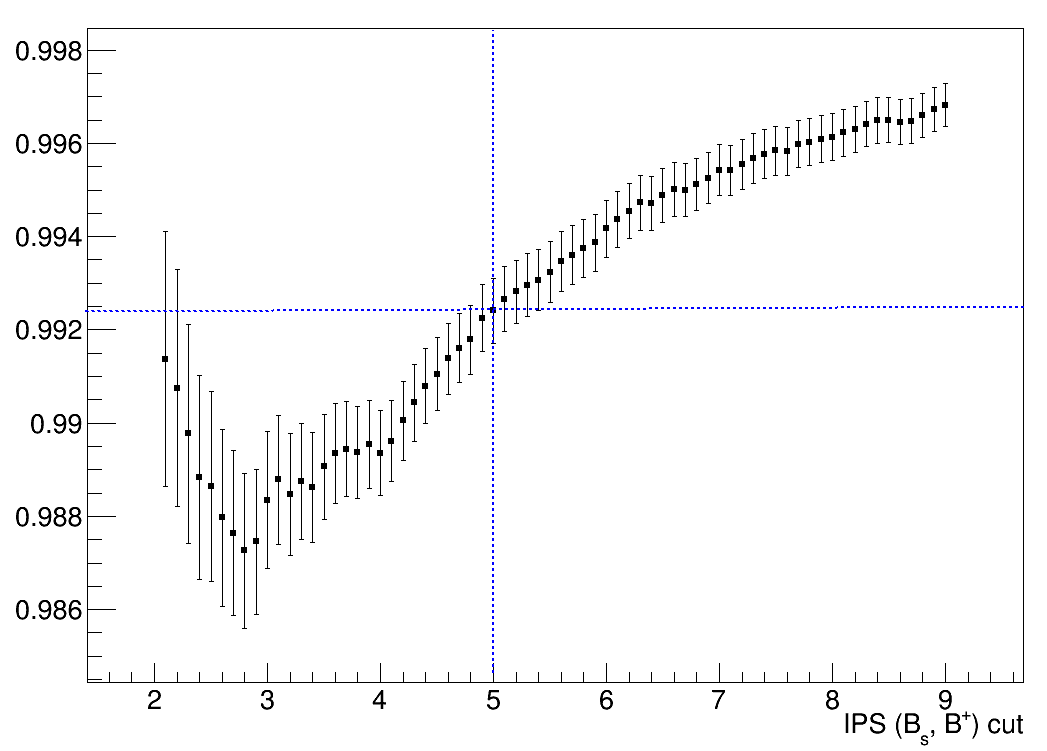
\includegraphics[width=\textwidth]{./Figs/Selection/IPS.png}
        \caption{ }
        \label{fig:IPS_ratio}
    \end{subfigure}
    ~ %add desired spacing between images, e. g. ~, \quad, \qquad, \hfill etc. 
      %(or a blank line to force the subfigure onto a new line)
    \begin{subfigure}[b]{0.4\textwidth}
        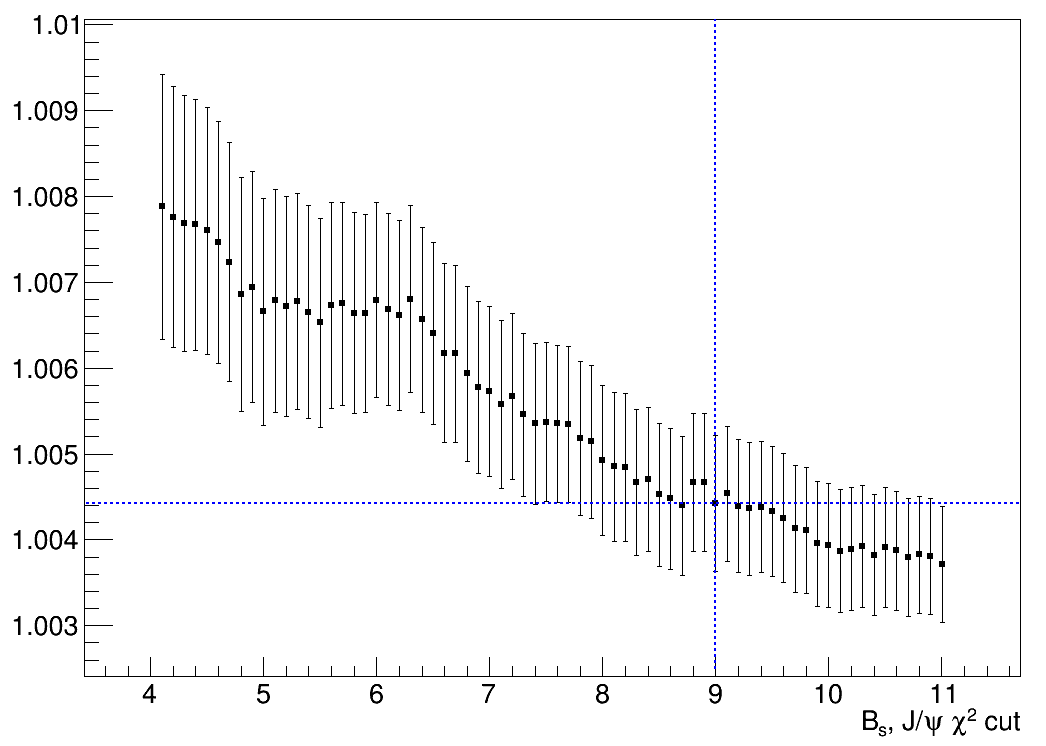
\includegraphics[width=\textwidth]{./Figs/Selection/CHI2.png}
        \caption{ }
        \label{fig:CHI2_ratio}
    \end{subfigure}
    ~ %add desired spacing between images, e. g. ~, \quad, \qquad, \hfill etc. 
    %(or a blank line to force the subfigure onto a new line)

    \begin{subfigure}[b]{0.4\textwidth}
        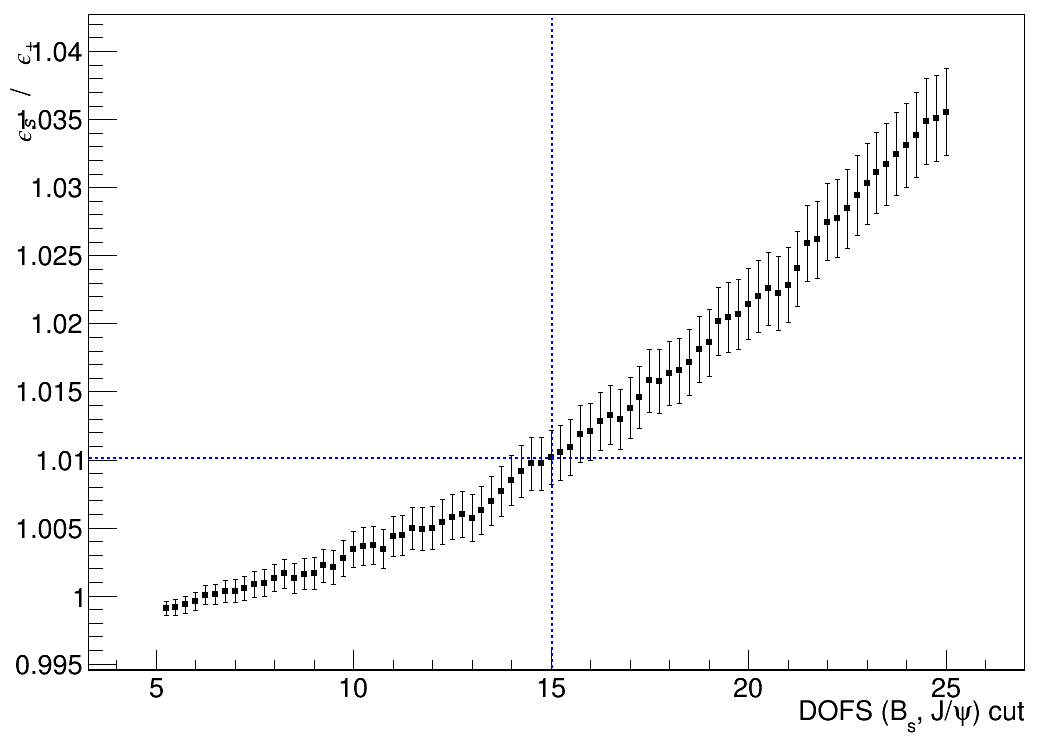
\includegraphics[width=\textwidth]{./Figs/Selection/DOFS.png}
        \caption{ }
        \label{fig:FD_ratio}
    \end{subfigure}
   \begin{subfigure}[b]{0.4\textwidth}
        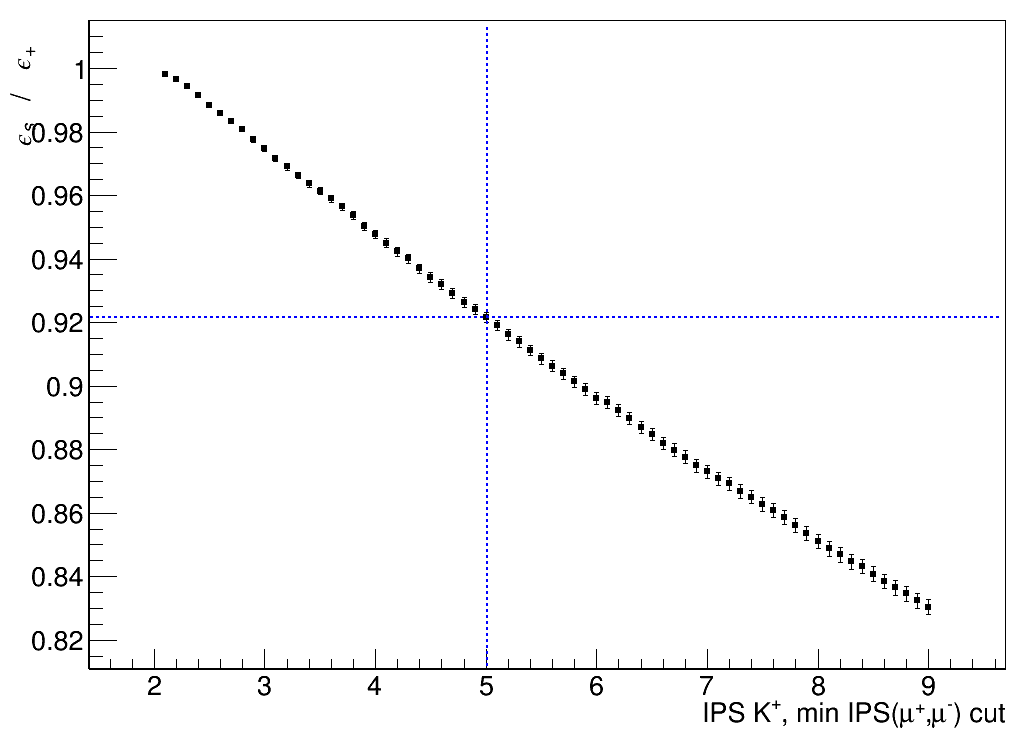
\includegraphics[width=\textwidth]{./Figs/Selection/daug_IPS.png}
        \caption{ }
        \label{fig:IPS_ratio}
    \end{subfigure}
    \caption{The ratio of $B^{0}_{(s)}\to\mu^{+} \mu^{-}$ to $B^{+}\to J/\psi K^{+}$ stripping efficiencies on MC events when each cut has been applied independently of all other cuts. The current cut values are marked by the blue lines.}
    \label{fig:ratio_plots}
\end{figure}



\begin{figure}
    \centering
    %\begin{subfigure}[b]{0.4\textwidth}
        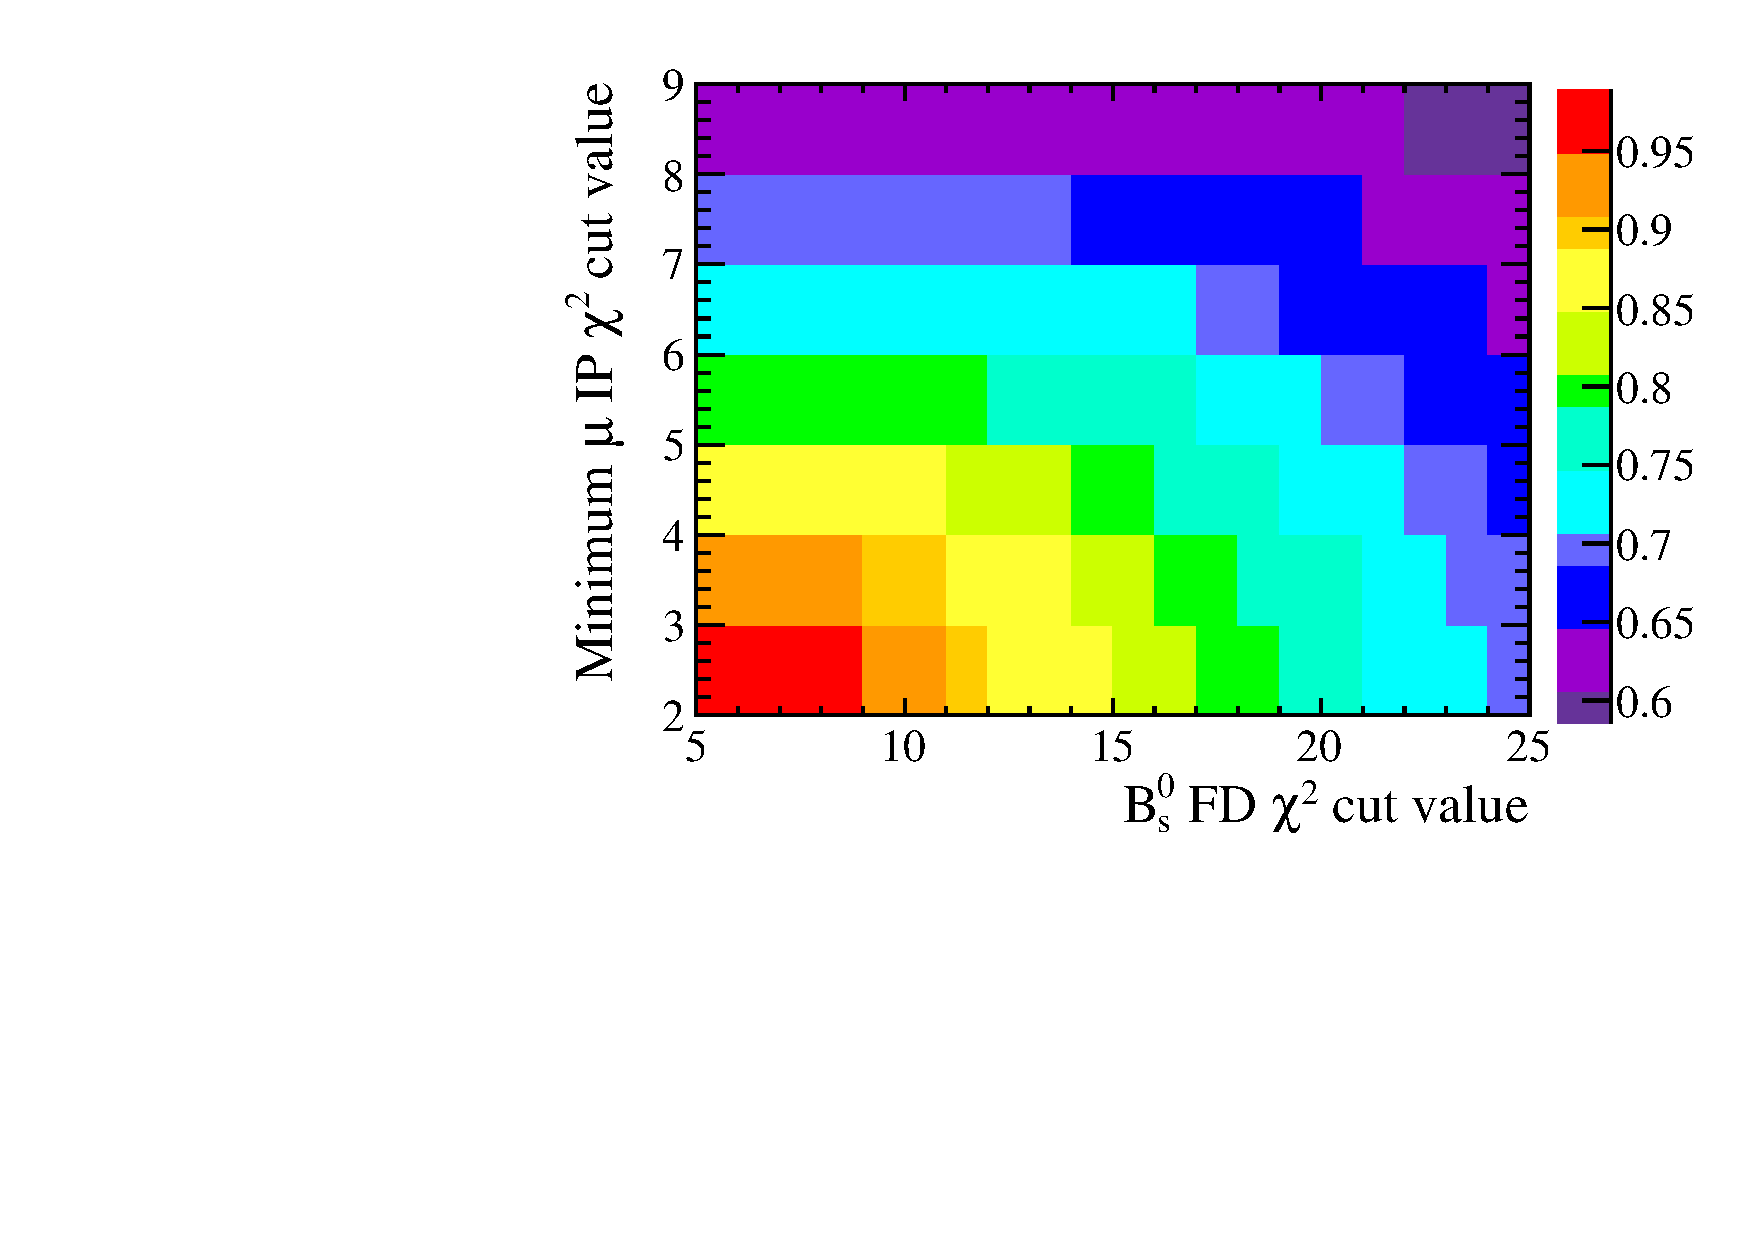
\includegraphics[width=\textwidth]{./Figs/Selection/eff_chart_pdf.pdf}
       % \caption{ }
      %  \label{fig:eff}
  %  \end{subfigure}
    ~ %add desired spacing between images, e. g. ~, \quad, \qquad, \hfill etc. 
      %(or a blank line to force the subfigure onto a new line)
   % \begin{subfigure}[b]{0.4\textwidth}
       % 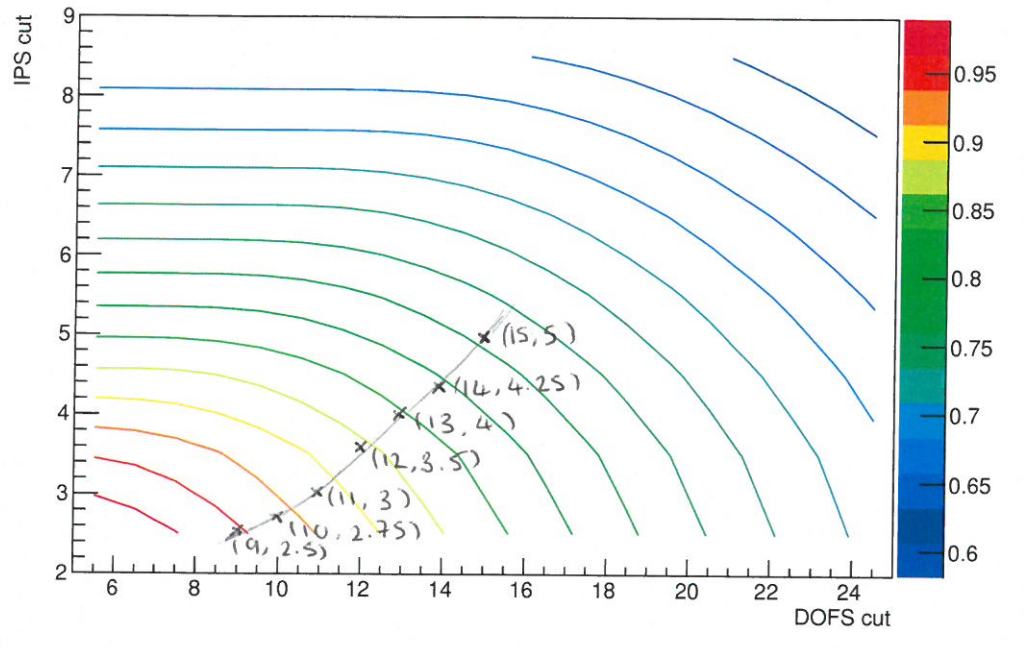
\includegraphics[width=\textwidth]{./Figs/Selection/strip_chart1.png}
      %  \caption{ }
      %  \label{fig:eff_contours}
  %  \end{subfigure}
    \caption{Efficiency figures.}
    \label{fig:efficiencyplots}
\end{figure}

\afterpage{
\begin{landscape}
\vspace*{\fill}
\begin{table}[htbp]
\begin{center}
\begin{tabular}{ ll|lll|lll}\hline
                       &                     & \multicolumn{3}{c}{Stripping line efficiency} &  \multicolumn{3}{c}{Stripping line retention} \\
\cline{3-8}
\bsd, \jpsi FD \chisqd & \mu, $h$ IP \chisqd & \bsmumu & \bdkpi   & \bujpsik & \bsmumu & \bdkpi & \bujpsik \\
\hline
15                     &5.00                 & XX $\%$ &  XX $\%$ &  XX $\%$ &  XX      & XX     & XX        \\
14                    &4.25                  & XX $\%$ &  XX $\%$ &  XX $\%$ &  XX      & XX     & XX        \\
13                    &4.00                  & XX $\%$ &  XX $\%$ &  XX $\%$ &  XX      & XX     & XX        \\
12                    &3.50                  & XX $\%$ &  XX $\%$ &  XX $\%$ &  XX      & XX     & XX        \\
11                    &3.00                  & XX $\%$ &  XX $\%$ &  XX $\%$ &  XX      & XX     & XX        \\
10                    &2.75                  & XX $\%$ &  XX $\%$ &  XX $\%$ &  XX      & XX     & XX        \\
9                     &2.50                  & XX $\%$ &  XX $\%$ &  XX $\%$ &  XX      & XX     & XX        \\
\hline
\end{tabular}
\end{center}
\label{tab:eff_and_retention}
\vspace{0.7cm}
\caption{Retention of data and stripping line efficiencies. Efficiencies are \bdkpi but retention is \bhh because the stripping line selects all \bhh decays, $h$ is $K$ or $\pi$. }
\end{table}
\vspace*{\fill}
\end{landscape}
}

\subsection{Stripping selection and offline cuts}
\label{finalloosesel}
%The stripping selection requirements along with a number of other loose selection cuts to select \bmumu, \bhh and \bujpsik decays in 2011, 2012, 2015 and 2016 are shown in Table~\ref{tab:fullpreselection}. The selection includes the looser stripping cuts on the \bsd and \jpsi FD \chisqd and muon and hadron IP \chisqd. Additionally the selection of \bmumu decays includes the momentum, ghost track probabilty and decay time cuts made in the \bhh stripping line, but were absent in the \bmumu stripping line. Several cuts are included to remove specific background events, the mass requirement on \bmumu decays is tightened to ensure $B_{S}^{0}\to\mu^{+}\mu^{-}\gamma$ decays are not within the mass window and a lower bound is placed on the $B$ meson transverse mometum to remove pairs of muons originating from $pp \to p\mu\mu p$ decays. %Something about that decays with mass above 6000 MeV are used for background studies?
%The decays that pass the selection cuts in Tables~\ref{tab:fullpreselection} in both data and simulated events are used to develop tigher selection requirements. 

The complete list of selection cuts applied in the cut based selection to select \bsmumu and \bhh decays in Run~1 and Run~2 data are listed in Tables~\ref{}. The stripping selection cuts from Table~\ref{} are included with the $B$ mesons FD \chisqd and daughter IP \chisqd requirements updated to the looser values and the selection of \bmumu decays includes the momentum, ghost track probability and decay time cuts made in the \bhh stripping line, but were absent in the \bmumu stripping line.

Additional selection requirements are applied after the stripping to remove specific backgrounds. A lower bound is placed on the $B$ meson transverse momentum to remove pairs of muons originating from $pp \to p\mu\mu p$ decays and a \jpsi veto is used to remove backgrounds from \bcjpsimunu decays. The semi-leptonic \bcjpsimunu decays, where \jpsimumu, contribute to the background of \bmumu decays when a muon from the \jpsi forms a good vertex with the muon from the $B_{c}^{+}$ decay. Due to the high mass of the $B_{c}^{+}$ this could place mis-reconstructed candidates within the \bs mass window. A `\jpsi veto' can be used to remove background events from \bcjpsimunu decays. The veto works by removing events where one muon from the \bmumu candidate combined with any other oppositely charged muon in the event has $|m_{\mu\mu} - m_{\jpsi}| < 30$~\mevcc. The veto has a rejection power of X  $\%$ on \bcjpsimunu events that have passed \bmumu selection cuts in Table~\ref{} and rejects only  $\%$ of \bmumu signal events. The expected number of \bcjpsimunu events after the full selection can be found in Section~X. 

The $B$ meson mass range for both \bsmumu and \bhh decays is narrower than the range in the stripping selection in Section~\ref{strippingold}. \bsmumu candidates are required to have a dimuon invariant mass greater than 5320 \mevcc. The motivation comes from mass fit studies that are detailed in Section X. The consequence of this cut is to remove \bdmumu decays, $B_{s}^{0} \to \mu^{+} \mu^{-} \gamma$ backgrounds and most backgrounds from mis-identified semi-leptonic and \bhh decays. The expect number of \bdmumu and mis-identified decays after the full selection can be found in Section~X. Similarly the \bhh mass window is reduced to remove contributions from mis-identified backgrounds. 

The selection applied to Run~1 and Run~2 is the same for all variables expect the track ghost probability and track \chisqd/ndof. Slightly looser cuts are used for Run~2 to take advantage to changes in the reconstruction that were introduced for Run~2. 

%\begin{landscape}
%\vspace*{\fill}
\begin{table}[htbp]
\begin{center}
\begin{tabular}{lll}
Particle                & \bsmumu                                     & \bhh                                 \\
\hline
\bs or $B^{+}$          & 5320 \mevcc $<$ M $<$ 6000 \mevcc           & 5100 \mevcc $<$ M $<$ 5500  \mevcc      \\                          
                        & DIRA $>$ 0                                    & DIRA $>$ 0                             \\
                        & FD $\chi^{2}$ $>$ 121                       & FD $\chi^{2}$ $>$ 121                  \\       
                        & IP $\chi^{2}$ $<$ 25                        & IP $\chi^{2}$ $<$ 25                   \\
                        & Vertex $\chi^{2}$/ndof $<$ 9                  & Vertex $\chi^{2}$/ndof $<$ 9              \\      
                        & DOCA $<$ 0.3 mm                             & DOCA $<$ 0.3 mm                          \\    
                        & $\tau$ $<$ 13.248 \ps                       & $\tau$ $<$ 13.248 \ps                \\
                        & $p_{T}$ $>$ 500 \mevc                        & $p_{T}$ $>$ 500 \mevc                \\

\hline
Daughter $\mu$ or $h$   & Track $\chi^{2}$/ndof $<$ 3 (4)               & Track $\chi^{2}$/ndof $<$ 3 (4)         \\                       
                        & Minimum IP $\chi^{2}$ $>$ 9                 & Minimum IP $\chi^{2}$ $>$ 9           \\             
                        & 0.25 \gevc $<$ $p_{T}$ $<$ 40 \gevc         & 0.25 \gevc $<$ $p_{T}$ $<$ 40 \gevc    \\
                        & $p$ $<$ 500 \gevc                             & $p$ $<$ 500 \gevc                       \\
                        & ghost probability $<$ 0.3 (0.4)             & ghost probability $<$ 0.3 (0.4)   \\
                        & $|$m_{\mu\mu} - m_{\jpsi}$| $<$ 30$~\mevcc        &$|$m_{\mu\mu} - m_{\jpsi}$| $<$ 30$~\mevcc    \\
                        & isMuon = True                               &  -                                \\

\hline

\hline
\end{tabular}
\vspace{0.7cm}
\caption{Selection cuts applied to select \bsmumu and \bhh decays, where selection is different between Run~1 and Run~2 the Run~2 values are shown in parenthesis next to the Run~1 values.}
\label{tab:fullpreselection}
\end{center}
\end{table}
%\vspace*{\fill}
%\end{landscape}



\subsection{Particle Identification}
\label{sec:PID}
%Not a fan of this section :(
Particle identification (PID) variables are used to refine the selection of \bmumu candidates and to separate different \bhh decays. 

In the selection of \bmumu decays PID variables are particularly useful to reduce the backgrounds coming from mis-identified semi-leptonic decays and \bhh decays and also help to reduce the number of combinatorial background events. The semi-leptonic decays that contribute to \bsmumu backgrounds are \bdpimunu, \bsKmunu, \bpimumu, \bdpimumu and \bcjpsimunu where \jpsimumu.

The PID requirements to select \bmumu decays are shown Table~\ref{} alongside requirements to separate different \bhh decays. Two types of PID variables, defined in Section~\ref{PID_variables}, are used; DLL variables and ProbNN variables. 

%A linear combination of ProbNN variables is used to select \bsmumu decays and remove semi-leptonic backgrounds. 
A linear combination of ProbNN variables is used to select \bsmumu decays and remove semi-leptonic backgrounds, in addition to the isMuon requirement applied in the stripping selection.
The classifiers used in ProbNN variables are tuned to give the best performance depending on the different data taking conditions in the detector for each year. %The efficiency of a cut on the linear combination of ProbNN variables to select \bsmumu decays and to reject background decays depends on the ProbNN tune being used. 
Since different tunes are used to select \bsmumu decays in 2016 data compared to Run~1 and 2015 data, the requirement on the linear combination of ProbNN variables varies with the year of data taking. The cuts are chosen to give similar efficiencies for each data sets at selecting signal and removing background across the different years. 



The separation of different \bdkpi and \bskk decays is done via DLL variables. These are useful to separate \bhh decays where $h$ is either a pion or kaon because the variables compare different particle hypotheses with the pion hypotheses. The selection requirements used are the same for each year of data taking.

\afterpage{
\begin{landscape}
\vspace*{\fill}
\begin{table}[htbp]
\begin{center}
\begin{tabular}{lll}
Decay                    & Particle               & PID requirements \\
\hline
\bsmumu  (Run~1 and 2015) & $mu^{+}$ and $\mu^{-}$ & ProbNN$\mu$ * (1 - ProbNN$\pi$) * (1 - ProbNN$p$) > 0.2 \\
\bsmumu  (2016)          & $mu^{+}$ and $\mu^{-}$ & ProbNN$\mu$ * (1 - ProbNN$\pi$) * (1 - ProbNN$p$) > 0.4 \\
\bdkpi and \bskpi       & $K^{+}$                & DLL$_{K\pi}$ $>$ 10 \\
                         & $\pi{-}$              & DLL$_{K\pi}$ $<$ -10 \\
\bskk                    & $K^{+}$ and $K^{-}$    & DLL$_{K\pi}$ $>$ 10 \\
\hline
\end{tabular}
\vspace{0.7cm}
\caption{Particle identification requirements to select \bsmumu decays and to separate the \bhh decays \bdkpi and \bskpi from \bskk. }
\label{tab:PID}
\end{center}
\end{table}
\vspace*{\fill}
\end{landscape}
}

%Tighter PID requirements are used to select \bmumu decays for the Branching Fraction measurements compared to those used for the effective lifetime measurement. This is because more mis-identidied decays extend in to the \bd mass window than the \bs mass window therefore tigher requirements are necessary to reduce them to an acceptable level. %However this also reduces the efficiency for selecting \bmumu decays. 

%{\it Prehaps a better way for the PID is to put the requirements in the text because the is could be clearer or maybe have two tables one for bsmumu and one for bhh? Also another consideration prehaps it would be clearere to seperate the effective lifetime and the BF after the stripping selection. I could clearly explain that the stripping and loose selection is used for both and therefore the BF decays must be considered in the stripping selection but after that the selection will focus on the effective lifetime. }



\section{Multivariate Classifiers}
\label{sec:MVC}

The selection described so far remove a large number of background candidates however because \bsmumu decays occur very rarely the data is still dominated by long lived combinatorial background from \bbbarmumux decays. To increase the signal purity of the data multivariate classifiers are used to separate signal from background events. 

A multivariate classifier is an algorithm that learns differences between signal and background candidates in the following manner, firstly the classifier is given two input samples, one contain only signal decays and the other containing just background decays and a set of input variables. These input variables have different distributions for signal and background events. Then the classifier uses the distributions of the input variables with its knowledge of which events are signal and background to learn the difference between the two types of events. Finally the algorithm is then be applied to a data set containing an unknown mixture of signal and background events and distinguish between them. For each event the algorithm produces a number, typically between -1 and +1, where high numbers indicate signal-like candidates and low numbers indicating background-like candidates. A cut is placed on the output of the classifier to remove background events with a classifier response less than a particular value and the remaining data set has a higher purity for signal events.

Two multivariate classifiers are used to select \bsmumu decays. Both classifiers are a type called Boosted Decision Trees (BDT) that are described in Section~\ref{sec:GeneralBDT}. A range of different classifiers were investigated but BDTs preformed the best at separating signal and background candidates. 

The first classifier (Sect. X), called the BDTS, is used to remove candidates that are very unlikely to be signal and is has  high efficiency to select \bsmumu decays. The second classifier (Sect. X), called simply the global BDT, is the final step in the selection process, the output is used to remove almost all remaining background candidates and has much lower efficiency to select signal events compared to the BDTS. The cuts applied to the output of this classifier is optimised to give the lowest expected uncertainty on the measurement of the \bsmumu effective lifetime (Sect. X).

Both classifiers were developed for the measurement of the \bmumu Branching Fractions. In the selection \bsmumu decays for this analysis the second classifier is used to classify candidates into 8 bins containing increasing proportions of signal candidates, not candidates are removed based on the output of the second BDT. Therefore the BDTS is necessary to reduce the number of background events to a more manageable level. The use of a single classifier was investigated to select candidates to measure the \bsmumu effective lifetime however it was found that the two classifiers developed for the Branching Fraction measurement performed best. 

\subsection{Boosted Decision Trees}
\label{sec:GeneralBDT}
A BDT is made up of the combined outputs of separate decision trees. A decision tree begins with a data sample, where each candidate is know to be signal or background and a set of variables describing these events. The decision tree applies a cut on a variable that will be the most effective at separating the signal and background in the sample and creates two sub-samples. Another cut is then applied on each of the sub-samples to further separate signal from background. This process is repeated until either a certain number of cuts, defined as the depth of the tree, or the number of candidates in each sub-sample has reached a minimum number. Each sub-sample produced at the end of the tree is called a leaf. The tree then uses the knowledge of which candidates are signal or background to assign a value of +1 or -1 to every candidate. A candidate is given a value +1 if it is in a leaf where the majority is signal and the value -1 if it is in a leaf that has a majority of candidates are background. The final decisions made by the tree are not prefect, some signal (background) events will be mis-classified as background events and given the value of -1 (+1). 

One decision tree on its own is often not particularly good at classifying events, there is no way to correct mis-classified events in the leaves, and it is particularly sensitive to statistical fluctuations in the training samples. A BDT combines the output of numerous decision trees to improve the classification of events and reduce the dependance of the final decisions on statistical fluctuations. A BDT starts with one decision tree and then assigns weights to events in the sample depending on whether the output of the decision tree classified the events correctly or incorrectly. The weighted sample is then used as the input for the training of the next decision tree. The weights are designed so that the next tree is more likely to correctly classify previously mis-classified events. This process is repeated until a certain number of trees have been trained. The re-weighting process is known as boosting and the weights applied to the samples are taken into account when combining the output of each decision tree into the overall output of the BDT. The output of a BDT will be a number between -1 and +1 where high numbers indicate signal-like candidates and low numbers indicating background-like candidates.


The TMVA package is use to develop and train the BDTs, the package provides several different methods of boosting that can be used. The adaptive boosting method was found to produce the most effective BDT.
This method of boosting assigns events incorrectly classified by one tree the weight, $w$, before being used in the input signal and background samples to the next decision tree. The weights assigned are given by
\begin{equation}
w = \frac{1 - f}{f}\text{, where } f = \frac{\text{Total misclassified events}}{\text{Total events}}.
\end{equation}
Therefore incorrectly assigned candidates are given a higher weight than correctly classified candidates. The `speed’ at which the boosting occurs is controlled by a the parameter $\beta$ where $w \rightarrow w^{\beta}$, this can be specified in the training of the decision tree, a large number of boosting steps can improve the performance of the BDT.
 %READ WHAT SIMON WROTE BECAUSE I DON’T UNDERSTAND TMVA! :( , in the adaptive boosting method the weight assigned during
%{\bf This is only really relevant if I describe the BDT training that I did. Start:}

The ability of a BDT to correctly identify signal and background candidates depends on three main factors;
\begin{itemize}
\item the size of the training samples - a large training sample is useful to prevent the BDT from being sensitive to statistical fluctuations and contains more information the classifier can use to learn the difference between signal and background
\item the input variables - different distributions in the input variables for signal and background candidates enable the classifier to easily separate the types of candidates, the overall performance is insensitive to poorly discriminating variables that are included
\item parameters that dictate the BDT training - the training of a BDT is specified by several parameters; the number of trees (NTrees), the tree depth (MaxDepth), the minimum number of events a leaf can contain (nEventsMin or MinNodeSize);, the `speed’ at which the boosting occurs and the number of cut values that a tree tries for a variable before making a decision (nCuts).
\end{itemize}

These three factors affect the performance of the BDT however the importance of each varies but together they can be used to prevent overtraining of the BDT. Overtraining is when the BDT is very sensitive to the statistical fluctuations in the training sample and is extremely accurate at classifying the candidates in the training sample by preforms poorly at classifying candidates in a statistically independent sample. Although this is less common in BDT than single decision trees, it can be avoided by having a sufficiently large training sample or by limiting the depth of trees or the number of trees in the BDT. 

%{\bf End.}


%\begin{equation}
%\alpha = ???
%\end{equation}

%where. Therefore incorrectly assigned candidates are given a higher weight than correctly classified candidates. The `speed’ at which the boosting occurs is controlled by a the parameter $\beta$ where $\alpha \rightarrow \alpha^{\beta}$, this can be specified in the training of the decision tree, a large number of boosting steps can improve the performance of the BDT.


%\subsection{Training signal and background samples}
%Simulated \bsmumu and \bbbarmumux decays are used to provide large signal and background training samples for both BDTs. In data \bsmumu candidates in the mass range 5431 to 6550 \mevcc consist almost entirely of \bbbarmumux decays, however the number of candidates in this mass range is too small to be a useful as sample of background candidates to train a BDT with comparable preformance to one trained entirely on simulated decays. 
%The simulated sample \bbbarmumux decays corresponds to the background expected with 7~\fb of data from $pp$ collisions at $\sqrt{s}$ = 8~\tev. The production of such a large sample requires a lot of space to be saved, therefore several measures were taken to reduce the size needed to save the simulated \bbbarmumux decays. The cuts, listed in Table~\ref{tab:MC_decays}, were applied to the simulated decays as they were generated to reduce the number of events saved on disk. Also the stripping selection cuts in Table~\ref{tab:PreviousStripping} were applied and candidates that did not pass the stripping selection were not saved. Unfortunately the \bbbarmumux sample therefore does not include candidates that are selected by the looser stripping selection described in Section~\ref{}. In order to gain the best BDT performance on data the same cuts should be applied to data that are applied to the samples used to train the BDT. Therefore the original cuts of and must be used to select \bsmumu candidates. 
%The complete list of selection requirements applied to the training samples used to develop both BDTs are listed in Table~\ref{}, the same selection is applied to \bsmumu and \bbbarmumux decays. %loose particle identification requirements are included to remove obvious background candidates. What exactly did Matteo apply, because Siim says bsmumu and bhh candidates are treated identically??
 
\subsection{The BDTS}
%The output of the stripping selection still includes many background decays, further cuts shown in Table~\ref{} reduce the background decays. Some selection cuts are designed to remove specific background decays and the selection for \bsmumu decays used in the Branching Fraction and effective lifetime analyses starts to diverge slightly.

%The BDTS is a multivariate classifier that is designed to reduce the number of combinatorial background events. It is a Boosted Decision Tree (BDT) (see Section~\ref{} for a detailed description) that is trained on \bsmumu and \bbbarmumux simulated decays that have passed the \bmumu selection requirements in Table~\ref{} and additional particle identification cuts listed in Table X. 
The BDTS uses input variables similar to those in the stripping selection to classify events;
\begin{itemize}
\item impact parameter \chisqd of the \bs
\item vertex \chisqd of the \bs
\item direction cosine of \bs
\item distance of closest approach of the muons
\item minimum impact parameter \chisqd of the muons with respect to all primary vertices in the event
\item impact parameter of the \bs, this is the distance of closest approach of the $B$ to the primary vertex
\end{itemize}
The signal and background samples used to train the BDTS are simulated \bsmumu decays and \bsmumu candidates in Run~1 data from the mass ranges 4800 - 5000 \mevcc and 5500 - 6000 \mevcc. The selection cuts listed in Table~\ref{tab:BDTSpresel} are applied to the training samples and the training parameters used in the BDT are listed in Table~\ref{tab:}. The output of the BDTS is flattened between 0 and 1 so that signal is uniformly distributed across the range and background is peaked at zero. The BDTS is applied to all candidates passing the \bmumu and \bhh stripping lines, and candidates are required to have a BDTS value above 0.05. The chosen cut value has a efficiency of X $\%$ on \bsmumu decays and reject X $\%$ of \bbbarmumux decays. This is illustrated in Figure X. 

\begin{table}[htbp]
\begin{center}
\begin{tabular}{ll}
\hline
\multicolumn{2}{c}{Selection applied to BDTS training samples.} \\ \hline
\bs FD $\chi^{2}$ $>$ 225 &$\mu^{\pm}$ $p_{T}$ $>$ 500 \mevc \\
\bs IP $\chi^{2}$ $<$ 25  & $\mu^{\pm}$ track $\chi^{2}$/ndof $<$ 3    \\
\bs Vertex $\chi^{2}$/ndof $<$ 9    &$\mu^{\pm}$ minimum IP $\chi^{2}$ $>$ 25   \\
\bs DOCA $<$ 0.3 mm    & $\mu^{\pm}$ 0.25 \gevc $<$ $p_{T}$ $<$ 40 \gevc  \\
\bs $\tau$ $<$ 13.248 \ps  &$\mu^{\pm}$  $p$ $<$ 500 \gevc  \\
\bs $p_{T}$ $>$ 500 \mevc  &  \\ %\bs DIRA $>$ 0 &
\hline
\end{tabular}
\vspace{0.7cm}
\caption{Selection cuts applied to select candidates for signal and background samples used to train the BDTS.}
\label{tab:BDTSpresel}
\end{center}
\end{table}

\begin{table}[htbp]
\begin{center}
\begin{tabular}{ll}
\hline
Parameter & Value \\ \hline
nTrees & 250 \\
nEventsMin & 400 \\
MaxDepth & 3 \\
%NNodesMax = 100000 \\
$\beta$ & 1.0 \\
nCuts & 20 \\
\hline
\end{tabular}
\vspace{0.7cm}
\caption{Training parameters used to specify the train of the BDTS.}
\label{tab:BDTStrainingparams}
\end{center}
\end{table}

\subsection{Global BDT}
\label{sec:globalBDT}

The global BDT is the final step in selecting \bsmumu decays and it is ver effective at seperating them from long lived combinatorial background decays. The discrimintaing power schieved by the global BDT is mostly dependant on isolation variables. Isolation variables, or just isolations, provide a measure of how isolated or far away each muon from a \bsmumu candidate is from other track in the event. The tracks of the muons from a rel \bsmumu decays will be, in general, far from other trakcs in the event because the \bsmumu decays tree contains no other tracks apart from the muons. However combinatorial background arises from semi-leptonic decays therefore muon tracks are likely to be close to other tracks that have originated from the same decay tree as the muon. Various different definitions of isolations have been used acorss different experiments from D0 and CDF to ATLAS, CMS and LHCb. These variables are very useful in the selection of very rare decays like \bsmumu because they enable background to bve removed whilst keeping a high efficiency for signal decays.

Two isolation variables are used in the global BDT, one compares long tracks in the event to muons in \bsmumu candidates and the other compares VELO tracks in the event to the muons. The definition of the track types can be found in Section X. The isolation variables are built from the output of BDTs. For each type of track a BDT is trained on simulated \bsmumu and \bbbarmumux decays using a set of input variables that describe track and vertex properties. The BDT compares the $\mu^{+}$ from a \bsmumu candidate with all other tracks in the event, excluding the track of the $\mu^{-}$, and gives an output, {\it iso$_{\mu^{+}}$(track)}, for each possible $\mu^{+}$ - track pairing. The sample process is repeated for the $\mu^{-}$. The BDT is designed to produce high output values for muons from \bbbarmumux decays and a low value for muons from \bsmumu decays. The isolation variable of a \bsmumu candidates is then composed of the sum of the highest values of {\it iso$_{\mu^{+}}$(track)} and {\it iso$_{\mu^{-}}$(track)} for any tracks in the event. The input cariables used to the Long track and VELO track isolations are listes in Appendix~\ref{}. The seperation power of these isolations are shown in Figure~\ref{}. Full details of the isolation development can be found in~\ref{}.

The isolations are used along with five other varibles in the global BDT. The full list of input variables used are;
\begin{itemize}
\item Long tracks isolation
\item VELO tracks isolation
\item $\sqrt{\Delta \phi^{2} + \Delta \eta^{2}}$, where $\Delta \phi$ is the difference in azimuthal angles of the muons and $\Delta \eta$ the difference in the pseudorapidity of the muons
\item the smallest IP \chisqd with respect to the primary vertex of the \bsmumu of the muons
\item vertex \chisqd of the \bs
\item IP \chisqd of the \bs with respect to the primary vertex
\item angle between the momentum vector of the \bs and the vector connecting the production and decay vertices of the \bs
\end{itemize}

These variables were chosen by training a BDT beginign with the most discrimintaing variable, the Long track isolation, and adding variables to determine which improved the performance to the classifer. Only variables that improved the performance were included in the global BDT. The training parameters used in the BDT are listed in Table~\ref{}. These parameters were chosen by scanning across a range of variables and chosing those that gave the best performance. 


 %The global BDT was trained on simulated \bsmumu and \bbbarmumux decays with 2012 data taking conditions for the signal and background samples. The simulated decas had to pass the selection requirements listed in Table~\ref{}. Independant samples were used for training and testing the global BDT. 


Simulated \bsmumu and \bbbarmumux decays are used to provide large signal and background training samples for the global BDT. In data \bsmumu candidates in the mass range 5431 to 6550 \mevcc consist almost entirely of \bbbarmumux decays, however the number of candidates in this mass range is too small to be a useful as sample of background candidates to train a BDT with comparable preformance to one trained entirely on simulated decays. 
The simulated sample \bbbarmumux decays corresponds to the background expected with 7~\fb of data from $pp$ collisions at $\sqrt{s}$ = 8~\tev. The production of such a large sample requires a lot of space to be saved, therefore several measures were taken to reduce the size needed to save the simulated \bbbarmumux decays. The cuts, listed in Table~\ref{tab:MC_decays}, were applied to the simulated decays as they were generated to reduce the number of events saved on disk. Also the stripping selection cuts in Table~\ref{tab:PreviousStripping} were applied and candidates that did not pass the stripping selection were not saved. Unfortunately the \bbbarmumux sample therefore does not include candidates that are selected by the looser stripping selection described in Section~\ref{}. In order to gain the best BDT performance on data the same cuts should be applied to data that are applied to the samples used to train the BDT. Therefore the original cuts of and must be used to select \bsmumu candidates. 
The complete list of selection requirements applied to the training samples used to develop global BDT are listed in Table~\ref{}, the same selection is applied to \bsmumu and \bbbarmumux decays. Independant samples were used for training and testing the global BDT. 
 
In the same way as the BDTS the final output of the global BDT is flattened to have a response between 0 and 1 that is uniform for signal and the background peaks at zero. The flattening is important for the measurement of the \bmumu Branching Fractions where a simultaneous fit is applied to the dimuon invariant mass in bins of BDT, flattening the BDT output enavke bins containing equal proportions of signal decays to be easily created. 



\subsection{Global BDT cut optimisation}
\label{sec:globalBDToptimisation}
 A cut is place on the output of the global BDT to select \bsmumu decays to measure the \bsmumu effective lifetime, \tmumu. The motivation comes for the fit choice of how to extract the lifetime from the data set detailed in Section X. The cuts value is chosen to give the smallest expected statistical uncertainty on the measurement of \tmumu or \invtmumu. This is done by using toy experiments for the expected number of \bsmumu events and combinatorial background for different cuts on the global BDT output. 

The fit proceedure to extract the \tmumu from the data is described in depth in Chapter X. Briefly the strategy is firsly to perform and unbinned maxiumum likelihood fit to the dimuon invaraiant mass spectrum, where components for \bsmumu and the combinatorial background are included in the fit. The mass fit is used to compute sWeights using the sPlot method \cite{}. Then a maximum likelihood fit is prefmoned to the sWeighted decay time distribution to extract \tmumu and \invtmumu. 

The toy experiments used to chose the cut on the global BDT have the following structure, firstly the number of expected \bsmumu and combinatorial background events are generated using the expected mass and decay time probability density functions. Then the mass fit is performed to extract the sWeights so that the decay time fit to sWeighted decays can be done to extract \tmumu and \invtmumu. For each possible cut on the global BDT 10,000 toy experiments were performed to give the median expected uncertainty on \tmumu and \invtmumu for each BDT cut value. Full details of the toy experiment set up and the probability density functions used are given in Appendix X. 

The number of expected \bsmumu and combinatorial background events for diferent BDT cut values is derived from the expected number of decays passing in the all the selection cuts and BDT $>$ 0.55 for Run~1 and Run~2 data as described in Section X. These predictions assume the SM branching fraction for \bsmumu and are given in Table~\ref{}. Since the output of teh BDT is flattened the number of \bsmumu decays is evenly distributed across the BDT range, therefore the expected number of \bsmumu decays is straight forward to calculated for each BDT cut value. The numerb of combinatirual background decays expected after each BDT is is computed from simulated \bbbarmumux decays using the ratio
\begin{equation}
R = \frac{\epsilon(BDT > X)}{\epsilon(BDT > 0.55)}
\end{equation}
where $\epsilon(BDT > X)$ is the efficiency of the cuts BDT $>$ X. The full selection requirement are applied to the simulated decays before taking the effieicny. The ratios for the different cuts values are shown in Table~\ref{tab:EfficiencyRatioCombBG}. Simulated decays had to be used to compute the efficiencies rather than data because there were too few candidates left after the higher BDT cuts were applied to data to enable meaningful studies. 

The mass distribution of the combinatorial background is a decaying exponential, it was observed from the simualted \bbbarmumux decays that the slope of the mass dustrubution changed with the BDT cut value as illustrated in Figure~\ref{}. The change in slope is accounted for when generating events for the toy experiment by changing the slope parameter ($\lambda$) for each BDT cut. Table~\ref{tab:CBGSlopeBDT} shows the slope of the mass distibtuion for different BDT cuts values evealutaed from \bbbarmumux simulated decays.

The results from 10,000 toy experiments for BDT cut values every 0.05 in the range 0.4 - 0.65 are shown in Table~\ref{tab:selOptimisation} along with the expected number of \bsmumu and combinatorial background decays for each BDT cut value. The median uncertainty of the fit for \tmumu and \invtmumu are given along with the signal significance ($\mathcal{S} = S/\sqrt{S+B}$) for each BDT cut. The highest signal significance and lowest expected uncertainties occur for a BDT cut of 0.55, therefore this cut value is used to select \bsmumu decays. 


\begin{table}[ht]
\begin{center}
\begin{tabular}{|l|c|}
\hline
BDT1flat cut & $R_{\epsilon}$ \\ \hline 
0.40 & 8.69 \\
0.45 & 3.91 \\
0.50 & 1.91 \\
0.55 & 1.00 \\
0.60 & 0.55 \\
0.65 & 0.32 \\ \hline
\end{tabular}
\caption{The ratio of efficiencies of cuts on the global BDT to select \bbbarmumux decays relative to a cut of 0.55 on the global BDT. }
\label{tab:EfficiencyRatioCombBG}
\end{center}
\end{table}

\begin{table}[ht]
\begin{center}
\begin{tabular}{|l|c|}
\hline
BDT cut & $\lambda$ /c$^{2}$MeV$^{-1}$\\ \hline \hline
0.40 & -0.00114 $\pm$ 0.00028 \\
0.45 & -0.00129 $\pm$ 0.00041 \\
0.50 & -0.00132 $\pm$ 0.00060 \\
0.55 & -0.00004 $\pm$ 0.00089 \\
0.60 & -0.00000 $\pm$ 0.00114 \\
0.65 & -0.00024 $\pm$ 0.00122 \\ \hline
\end{tabular}
\caption{The slope of the combinatorial background mass distribution for different cut value on the global BDT evaluated from \bbbarmumux simulated decays.}
\label{tab:CBGSlopeBDT}
\end{center}
\end{table}

\begin{table}[ht]
\begin{center}
\begin{tabular}{llllll}
\hline
BDT cut & \bsmumu & Combinatorial & $S/\sqrt(S+B)$ &  $\sigma\left(\tauBsmm\right)$  & $\sigma \left( \invtauBsmm \right)$ \\ %& \invtauBsmm pull & \invtauBsmm pull  \\
        &         & background    & /$\ps$             & /$\ps^{-1}$  \\  \hline%& mean & width \\ \hline
0.40    &         &               & 3.87 & 0.345 & 0.128 \\ %& $-0.01 \pm 0.01$ & $1.020 \pm 0.007$ \\
0.45    &         &               & 4.51 & 0.309 & 0.114 \\ %& $-0.02 \pm 0.01$ & $1.014 \pm 0.007$ \\
0.50    &         &               & 4.85 & 0.291 & 0.108 \\ %& $-0.01 \pm 0.01$ & $1.029 \pm 0.007$ \\
0.55    &         &               & 4.94 & 0.285 & 0.106 \\ %& $0.00 \pm 0.01$ & $1.010 \pm 0.007$ \\
0.60    &         &               & 4.86 & 0.297 & 0.109 \\ %& $-0.02 \pm 0.01$ & $0.996 \pm 0.007$ \\
0.65    &         &               & 4.65 & 0.309 & 0.115 \\  \hline%&  $-0.01 \pm 0.01$  & $1.000 \pm 0.007$ \\ \hline
\end{tabular} 
\caption{ The number of expected \bsmumu and combinatorial background decays and the signal significance for each cut value in the global BDT and the \tmumu and \invtmumu results from 10,000 toy experiment for the expected number of events. }
\label{tab:selOptimisation}
\end{center}
\end{table}

%\section{Multivariate Classifier}
%\label{sec:BDT}
%After the selection described so far the data set still contains predonominately background decayse mostly from long lived combinatorial background from \bbbarmumux decays. The most effective way to remove the remaining background decays without comprimising on the efficiency to selection \bsmumu decays is to apply a cut on the output of a multivariate classifier.

%A multivariate classfier is an algorithm that leanrs differences between signa and background events in the following way; the classifier is gien tow input samples, one contain only signal decays and the other containing just background decays and a set of input variables. THese input variables have different distributions for signal and background events. The classifier uses the distributions of ths input variables with it's knowledge of which events are signal and background to learn the difference between the two types of events. The algorithm is then be applied to a data set containing an unknown mixture of signal and background events and distinguish between them.  For each event the algotithm produces a number typically between -1 and +1 with high numbers indicating signal-like events and low numbers indicating background-like events. A cut can then be places on the output of the classifier to remove background events with a classifer response less thatn a particular value and the remaining daata set has a high purity for signal events. 

%To seperate the signal \bsmumu decays from the background decays a type of classifer called a Boost Decision Tree (BDT) is used. Other types of classifers were investigated however their performance was not as good. A BDT is made up of the combined outputs of seperate decision trees. A decision tree begins with a sample of event, where each event is know to be signal or background and a set of variables descrubing these events. The decision tree applied a cut on a variable that will be the most effective at seperating the signal and background events in the sample and creates two sub-samples. Another cut is then applied on each of the sub-samples to futher seperate signal from background. This process is repeated until a certain number of cuts, defined as the depth of the tree, or the number of events in each sub-sample has reached a minumum number. Each sub-sample produced at the end of the tree is called a leaf. The tree then uses it's knowledge of whehter an event is signal or background to assign each event the value of +1 or -1. An event is given a value +1 if it is in a leaf that is made up of a majority of signal eventsand an event is given the value -1 if it is in a leaf that has a majority of background events. The final decisions made by the tree are not prefect, some signal (background) events will be mis-classified as background events and given the value of -1 (+1). The process of decision making is illustrated in Figure~\ref{}. 

%One decision tree on its own is often not particulary good at classifying events, there is not way to correct mis-classified events in the leaves, and it is particularly sensitive to statistical fluctuations in the training samples. A BDT combined the output of numerous decision trees to improve the classification of events and reduce the depandance of the final decisions on statistical flucuations. A BDT starts with one decision tree and it then assigns weights to events in the sample depending on whether the output of the decision tree classified the events correctly or incorrectly. The weighted sample is then used as the input for the training of the next decision tree. The weights are designed so that the next tree is more likely to correly classify previously mis-classified events. This process is repeated until a certain number of trees have been trained. The reweighting process is know as boosting and the weighted applied to the samples are taken into account when combining the output of each decision tree into the overall output of the BDT. 

%The preformance a BDT can acheive depends on three main factors;
%\begin{itemize}
%\item the size of the training samples avaliable, the larger the training sample the more information the BDT can use to correctly classify events
%\item the input variables used to makes each decision in the trees - variables that have distinctly different distributions for signal and background events enable the classifier to split samples into sub samples with a high signal or background purity. (Also something about correlations?)
%\item the parameters that guide the training of the trees, such as the depth or miniumum number of events allowed in the leaves and the speed at which boosting occurs and also the total number of trees.
%\end{itemize}


%The preformance of a classifer depends on these three inputs in different ways but together they must be used to avoid overtraining of the algorthm. Thsi occurs when the final algorithm is extremely sensitive to statistical flucutations in the training samples and therefore preforms poorly when used on a statistically indpenedant set of events. Overtraining can be avoided by using a very large training sample and by limiting the number of trees in the BDT or the depth of each tree. Overtraining can be checked for by testing and training the algorithm on seperate samples. 


%(I think that before re-writing this section I should read the TMVA guide again, all the BDT parts both on boosting and also about what a BDT is it will given me good information to include and it also explains varibles such as nCuts. Why didn't I read that earlier?!? It also explains how a BDT is in sensitive to poorly discriminating variables and also how variables are ranked from the output of the BDT which will be useful when I explain how I chose the input variables. Prehaps once I have this chapter I should work out what key points I want to say where and they write again! But sometimes it is only through writing you can work this out. But then prehaps it should be; 1. short bullet points, 2. detailed bullet points and checking the order, 3. write!)

%The TMVA package was used to build several BDTs with different boosting techniques. The training and testing of the BDTs using adaptive boosting, gradient boosting and a novel uBoost methog is discussed in the following sections. The uBoost method is a novel method of boosting that creates an output with a uniform efficiency for a specific input variable that is not used in the training. This is particularly interesint for the measurement of the effective lifetime. The BDT output could be required to be uniform in the decay time which would simplify understanding the efficiency as it vaired with the decay time. This is discussed futher in another section. Other boosting methods were considered but didnot preform as well as the adaptive or gradient boosting or offer the novel method of the uBoost algorithm.

